\chapter{仿冒开发者行为特征实证分析}
\label{chp:discoveries_behavior}

本章针对仿冒应用开发者的行为特征进行实证研究,内容主要针对仿冒应用开发者在各市场的投放频率、仿冒应用的投放方式等行为进行研究,了解该类行为有助于市场方与一般应用开发者对抵御仿冒应用作者的攻击。
本章实证研究从三部分展开,结合应用证书视角与结合时间维度视角对仿冒应用开发者的行为进行分析,对应以下三个研究问题:

\begin{itemize}
    \item RQ4:仿冒应用与开发者的对应关系如何?
    \item RQ5:仿冒应用证书可以活跃多长时间?
    \item RQ6:仿冒应用的投放是否有规律?
\end{itemize}

\section{研究方法}

本节介绍本章研究中整理研究数据的方法,以讨论研究的结构有效性。
对RQ4,根据~\autoref{sec:signature}的介绍,可利用样本的应用证书构建其与应用作者的对应关系,RQ5亦涉及应用证书相关信息使用,因此需要阐明应用证书数据的获取方式;
同时,RQ5有对应用证书活跃时间的需求,本章研究引入了一个应用证书活跃时间的近似计算方法;
对RQ6,为研究仿冒引用的投放规律,本研究整理复原了各款正版应用各版本上架的时间线,本节将介绍时间线的整理方法。
本章研究对象为与上一章相同、由69,414个正版样本与52,638个仿冒样本组成的应用集。

由~\autoref{sec:signature},可知每个APK文件内都有包含应用开发者信息的\textit{CERT.RSA}文件。
每个仿冒样本,作者将其解压,取出\textit{/META-INF}文件夹中的应用证书文件,再利用Keytool~\cite{keytool}工具获取证书信息(如\textit{应用证书SHA1码}与\textit{应用开发者名})。
Keytool工具为Java自带工具,被广泛地用于管理密钥和证书,因此可相信使用Keytool获取的应用证书信息无误。

在获取应用证书活跃时间方面,由于Janus类似一个爬取各大市场应用的平台,并不能感知某样本的下架时间或某样本是否已下架,因此只能对仿冒应用证书的活跃时间作近似计算。
计算的具体方法为将所有仿冒样本遍历一次,取出样本的应用证书SHA1码,凭借该样本的搜集时间更新该应用证书的最早出现时间(或最晚出现时间),取各证书最早出现时间与最晚出现时间为证书的活跃期,活跃期长度则为该证书的活跃时长。

为了解仿冒应用的投放速度,研究需要获取各款目标应用每个版本的更新时间和与该版本对应的仿冒样本的上架时间。
各个目标应用多年来发布版本众多,已无法从大部分应用官网中寻回完整更新日志,因此本研究借助样本集中的正版样本搜集时间整理复原各版原版应用的上架时间线。
本文对所有收集到的正版样本按目标应用进行分类,再按照版本号对同一目标应用下所有样本排序。
由于同一应用可在多个市场上架,同一版应用在不同市场可能存在细小差别(如在华为市场上架的应用需要接入华为钱包作为支付途径),导致同一版本的APK安装包具有不同SHA1码,因此此处以应用版本而非应用SHA1码为粒度分割样本,以消除上述情况影响。
另外,基于各市场审核流程、其他商业因素考虑,可能存在应用同一版本在不同市场有不同上架时间的情况。
针对该情况,如某版原版样本存在多个上架时间,本研究只取最小值,该值表示仿冒应用开发者可接触该版原版应用的最早时间。
之后,将每款应用中每个版本上架时间串联,即可大致重现每款应用的更新时间线。


从仿冒样本角度考虑,仿冒样本大多不是重打包应用,无法与原版应用的版本号直接对应。
为求出仿冒样本的仿冒延迟(即原版应用上架时间与仿冒样本上架的时间差),本文提取出每个仿冒样本的上架时间,以不晚于这个仿冒样本发布的原版应用作为其对应的仿冒对象,取两者上架时间差作为仿冒延迟。

\section{实证研究流程与结果解析}

本节分为四个部分,前三个部分分别对应本章三个研究问题的研究流程,最后一部分对本章研究进行有效性分析。

\subsection{应用证书与仿冒应用对应关系}

\noindent{\bf RQ4:仿冒应用与开发者的对应关系如何?}

由于每个仿冒样本均有对应的应用证书,本研究构造了仿冒样本与应用证书的二分图,其中两类节点分别为仿冒样本和应用证书,若两节点之间存在边,则表示该样本由该证书签署。
在仿冒应用持有的所有应用证书中,多数证书(76\%)仅仅关联了一个或两个仿冒样本,与最多仿冒应用的证书签署了1,374个仿冒样本。
\autoref{table:certificate_number_statistic}统计了应用证书和他们对应的仿冒样本数量。
表格第一栏为仿冒样本的数量区间,第二栏为关联的仿冒样本数量该落于区间的应用证书数,如第一列数据指有8252个应用证书签署的样本数为1到5个。
大部分应用证书都只关联了1到5个应用样本,但也有少量应用证书与大量仿冒样本有关联关系。

\begin{table}[htbp]
    \renewcommand{\arraystretch}{1}
    \footnotesize
    \centering
    \caption{应用证书/仿冒应用数量对应表}
    \vspace{1mm}
    \begin{tabular}{l c c c c c c c}
        \toprule
        {\bf 关联仿冒样本数量} & {\bf 1-5} & {\bf 6-10} & {\bf 11-50} & {\bf 51-100} & {\bf 大于100} \\
        \midrule
        {\bf 应用证书数量}     & 8252      & 525        & 531         & 71           & 80            \\
        \bottomrule
    \end{tabular}
    \label{table:certificate_number_statistic}
\end{table}

鉴于应用证书与应用开发者存在多对一关系(\secref{sec:signature}Android App签名机制),作者认为每个应用证书只签署少量样本是仿冒应用开发者规避应用市场监管机制的策略。
如果仿冒应用开发者只使用一个应用证书上传多个仿冒应用,万一其中一个应用被投诉下架,使用同一证书签署的其他的应用很可能会受到牵连。
但一个仿冒应用开发者可持有多个应用证书,即仿冒应用开发者可利用多个身份在应用市场中上传应用,继而令应用市场就难以找到仿冒应用之间的关联。
即使其中一个证书签署的仿冒应用被举报下架,由其他证书签署的余下应用也得以被保全。

另一方面,有部分仿冒应用应用证书关联着多个仿冒样本。
其中,SHA1码为``\emph{61ed377e85d386a8dfee6b864bd85b0bfaa5af81}''的应用证书是所有证书中关联仿冒样本最多的,有1,374个样本由该应用证书签署。
不仅如此,该应用证书还是其中一个在应用市场中活跃时间最长的应用证书。
本研究采用的应用集上架时间范围为2015年5月29日至2018年9月15日之间,使用上述证书签署的样本最早于2015年11月12日在百度手机助手上架,最晚于2018年9月15日在百度手机助手上架。
2015年至2018年间,该证书一直处于活跃状态,29个渠道中,除Uptodown,天翼应用市场、Apkpure、GiONEE、中移动应用商店、Google Play应用商店6个应用市场中未有发现由该证书签署的样本外,其他23个应用来源均有发现与该证书关联的样本,样本涵盖了本研究数据集47个目标应用中的37个(79\%)。

然而,三年期间发布1,374个样本是有违常理的。
以一年365天计算,若上述证书由某一个人或组织持有,则平均该个人或组织平均每1.25日需开发出一个新应用样本,该开发速度与日常认知并不一致。
利用Keytool从该证书抽取出的开发者信息,发现开发者名为``Android'',经查证,该证书为Android Studio自带的Android调试证书~\cite{UICC_cert}。
该结果表明国内大部分应用市场在审核阶段并未对该类证书进行有效拦截,开发者可凭借该类证书将仿冒应用上传至市场中,增加用户风险。

进一步,作者抽取所有证书的开发者名称进行匹配,得到~\autoref{table:certificate_developer_name}。
与下文~\autoref{table:certificate_number_statistic}相似,表格第一栏为某开发者名对应应用证书的数量区间,第二栏为对应应用证书数量该落于区间的开发者名称数,如第一列数据指有5355个开发者名称仅与1个应用证书对应。

\begin{table}[htbp]
    \renewcommand{\arraystretch}{1}
    \footnotesize
    \centering
    \caption{应用证书数量/开发者名称数量对应表}
    \vspace{1mm}
    \begin{tabular}{l c c c c c c c}
        \toprule
        {\bf 对应应用证书数量} & {\bf 1} & {\bf 2-5} & {\bf 6-10} & {\bf 11-50} & {\bf 大于50} \\
        \midrule
        {\bf 开发者名称数量}   & 5355    & 419       & 38         & 23          & 9            \\
        \bottomrule
    \end{tabular}
    \label{table:certificate_developer_name}
\end{table}

对应证书最多的前10个开发者名称与其对应证书数量依次为:\emph{cn}(873),\emph{Android Debug}(441),(空字符串)(279),\emph{Unknown}(207),\emph{mobcent}(195),\emph{addone}(125),\emph{Java}(102),\emph{Android}(63),\emph{1}(56),\emph{a}(43),其中\emph{Android Debug}、\emph{Android}为Android调试证书的开发者名,\emph{Java}很可能为利用Keytool生成证书的默认开发者名,空字符串、\emph{cn}与\emph{Unknown}为其他工具生成证书的默认开发者名(CN对应生成证书时需输入的开发者昵称,Common Name),\emph{1}、\emph{a}也不是有意义的开发者名称。
因此,除\emph{addone}与\emph{mobcent}两个开发者名称可能有具体含义外,余下8个开发者名称均很有可能为某些工具生成证书时采用的默认开发者名称,即其对应的应用证书很可能为调试证书。

\begin{table}[htbp]
    \renewcommand{\arraystretch}{1}
    \footnotesize
    \centering
    \caption{开发者名称/仿冒样本数量对应表}
    \vspace{1mm}
    \begin{tabular}{l c}
        \toprule
        {\bf 开发者名称}      & {\bf 对应仿冒样本数量} \\
        \midrule
        cn                    & 1888                   \\
        Android               & 1661                   \\
        Android Debug         & 1285                   \\
        (空字符串)          & 1278                   \\
        zh                    & 1176                   \\
        http://soft.sj.91.com & 1033                   \\
        yk                    & 982                    \\
        Gavin Van             & 698                    \\
        Unknown               & 653                    \\
        android               & 560                    \\
        \bottomrule
    \end{tabular}
    \label{table:developer_name_sample_cnt}
\end{table}

将开发者名称--应用证书--仿冒样本关联,可得到开发者名称与其对应的仿冒样本数量。
与最多样本关联的前10个开发者名称如~\autoref{table:developer_name_sample_cnt}所示。
综合以上几个表格,可确定国内各大应用市场并未对调试证书签署的应用进行拦截,从而产生十分大的安全风险。
此外,虽然~\autoref{table:certificate_developer_name}显示多数开发者名称与应用证书呈一对一关系,但该现象不与前文推论(仿冒应用开发者利用多个证书发布仿冒应用,每个证书只对应少量样本)矛盾,因为开发者在生成证书时可随意编写开发者名称,开发者名称与仿冒应用开发者之间对应关系并不明确。
相反,~\autoref{table:certificate_developer_name}中的\emph{addone}与\emph{mobcent}两个开发者名称分别对应证书125个和195个,对应样本数则分别为149个和263个,可为上述推论提供数据支持。

% \subsection{仿冒应用证书活跃时长}
% 从某个角度看,仿冒应用应用证书的活跃时长反映了应用市场的监管力度大小,也能反映市场之间在安全方面是否具有良好的合作机制。
% 所以本节有研究问题如下:

% % \noindent{\bf RQ 3.2} How long can a fake app's certificate survive?
% {\bf RQ 3.2}:一个仿冒应用开发者的应用证书可以活跃多久?

% 本文整理了不同仿冒应用应用证书的出现时间,得出了下面的结果:

% % \noindent{\bf Answer to RQ 3.2.} Fig.~\autoref{fig:Fake_certificate_survival_distribution} shows the distribution of the time a fake certificate can survive in markets.
% {\bf RQ 3.2. 结果}\autoref{fig:Fake_certificate_survival_distribution}展示了不同仿冒应用应用证书在应用市场里活跃时间的总体分布。
% % In the left density distribution subplot, $x$-axes is the latency and $y$-axes shows the probability density of data at corresponding $x$ value.
% 在左边的密度分布函数图中,$x$轴表示其活跃的时长,$y$轴则表示了与$x$轴上的值对应的概率密度。
% % The total area under the curve is 1, and the area under two $y$ values $y1$ and $y2$ is the probability of their corresponding value $x1$ and $x2$ account for in data.
% 曲线下的总面积为1,任意两个$y$值$y_1$、$y_2$之间的曲线下面积是其对应的$x$轴上的值$x_1$、$x_2$在数据中占有的概率。
% % For example, in Fig.~\autoref{fig:Fake_certificate_survival_distribution}, the area beneath curve between 0 to 200 on $x$-axes is close to 0.8, which means nearly 80\% of certificates only survive for no more than 200 days.
% 比如说,\autoref{fig:Fake_certificate_survival_distribution}中$x$轴从0到200之间的值对应的$y$轴曲线下方的区域面积接近0.8,意味着约80\%的仿冒应用应用证书不会活跃多于200天。

% % To judge how long a fake certificate can survive is similar to how we calculate the update frequency of an app, the first time and the last time a fake sample from the same certificate gets crawled are marked.
% 断定一个仿冒应用应用证书活跃市场的方法和前述计算应用更新频率的方法稍有类似,本文把某个应用证书关联的所有样本都找出来,提取出其中最早和最晚被爬取的样本的发布日期时间戳,然后将他们的差值的绝对值当作是这个应用证书的活跃时长。
% % The time when a sample was crawled from a market might be different from the time when it is available in the market, but our crawler downloads new samples from different markets by days and we also use days as the unit in our measurement, so we can approximately regard this two values as the same one.
% 从时长上爬取到样本的日期与样本在应用市场上实际能活跃的时间稍有不同,但由于Janus的爬虫工具每日都从应用市场中爬取样本,而本文并没有其他方法可以知晓某款App具体在应用市场中上架了多久,只能近似地将上述提到的时间差当作是某个应用证书能在应用市场上活跃的时间。

% \begin{figure}[htbp]
%     \centering
%     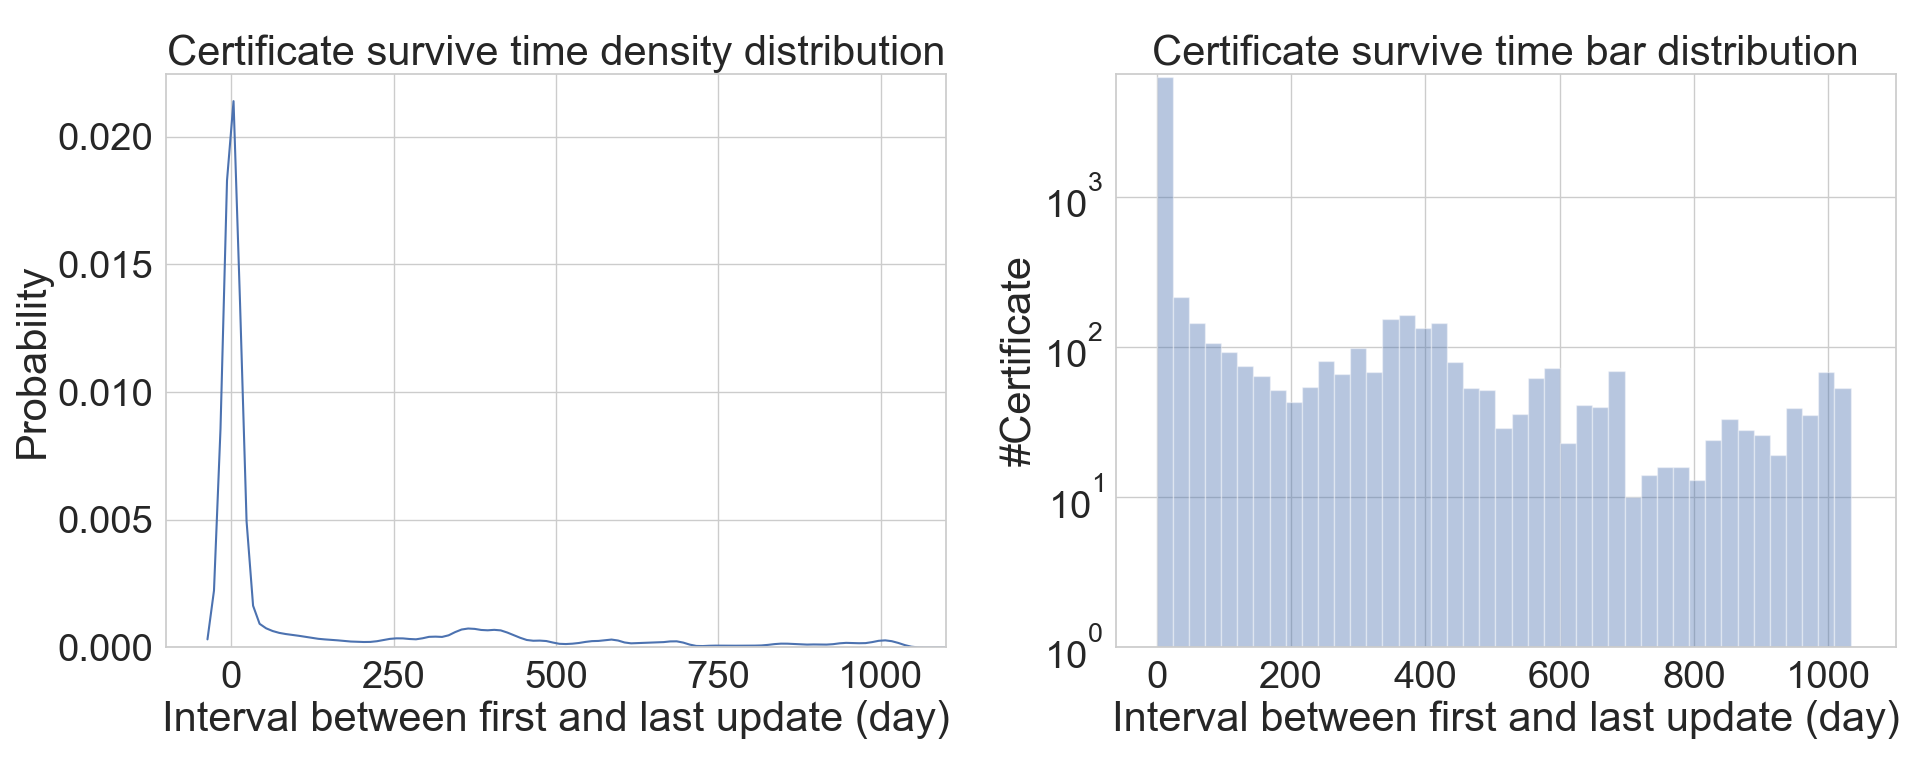
\includegraphics[width=\textwidth]{./Figures/edwin-Fake_certificate_survival_distribution2.png}
%     \caption{仿冒应用应用证书活跃时间分布}
%     \label{fig:Fake_certificate_survival_distribution}
% \end{figure}

% % As shown in Fig.~\autoref{fig:Fake_certificate_survival_distribution}, the distribution of fake certificate survival time shows that almost all the fake certificates live a short life, which means most fake certificates only show up in a short period of time.
% 正如\autoref{fig:Fake_certificate_survival_distribution}所示,仿冒应用应用证书活跃时间的分布表明几乎所有仿冒应用应用证书都只能活跃相当短的时间,这表明大多仿冒应用只会在一个很小的时间窗口里出现,然后迅速消失。
% % This can be explained by a scheme that most markets have.
% 这可以由大部分市场都有的一个安全机制解释。
% % Once an app is found malicious or illegal, the market would stop that specific developer from uploading more samples by refusing to receive samples with the same certificate.
% 只要一款App被发现具有恶意行为或者违法行为,应用市场就会禁止开发者再使用该证书上传应用,也就是常见的封号处理。
% % There are also a number of certificates which can survive for a long time.
% 但是,也有一部分的仿冒应用应用证书活跃了相当久的一段时间。
% % According to the figure, some fake certificates even traverse the whole study interval.
% 根据图表信息,可以看到有的仿冒应用应用证书的生命周期甚至贯穿了本文整个研究截取的时间周期。
% % We will conduct a case study on this phenomenon in Section ~\autoref{sec:casestudy}.
% 对于这个异常样本,本文会在后续的案例分析中有更详尽的案例分析。

% \begin{figure}[htbp]
%     \centering
%     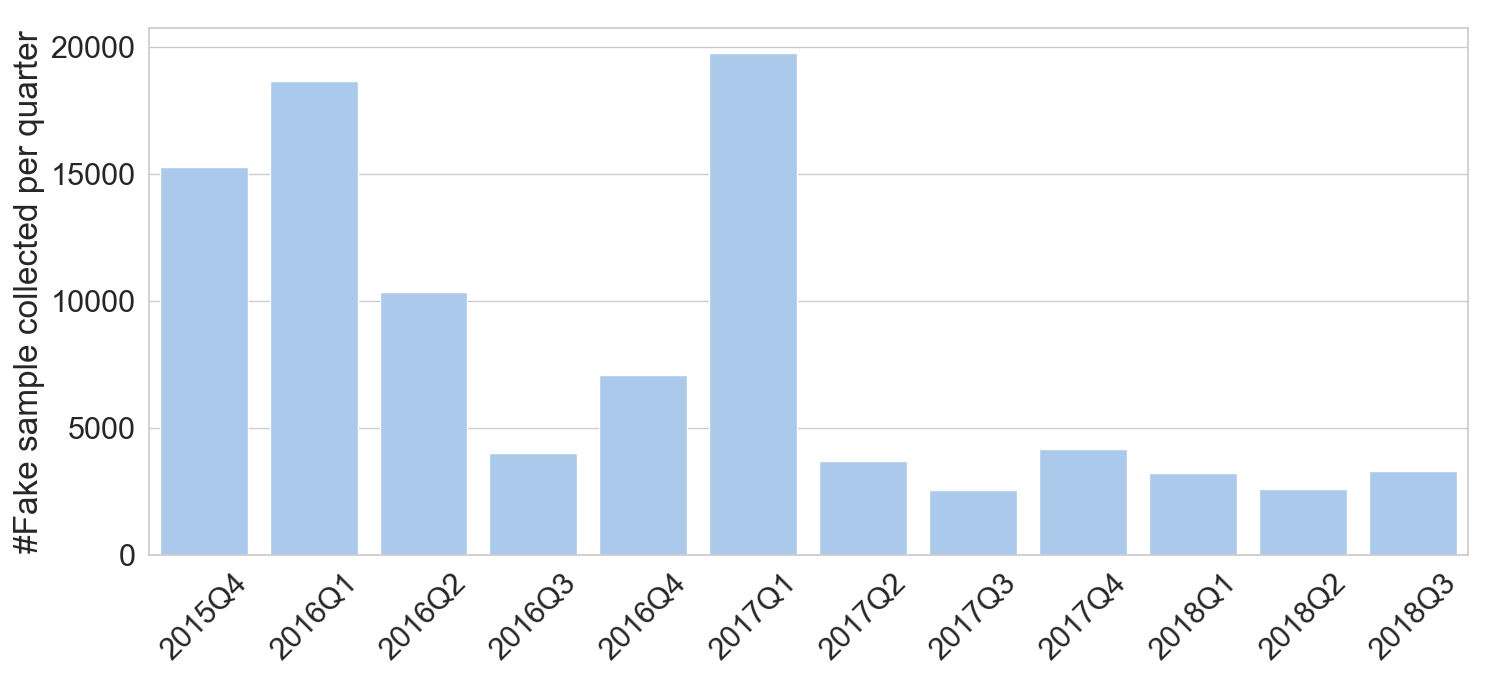
\includegraphics[width=\textwidth]{./Figures/edwin-Number_of_samples_collected_per_quarter_3.png}
%     \caption{每季度爬取到的仿冒样本数量(2015年第四季度到2018年第三季度)}
%     \label{fig:Number_per_quarter}
% \end{figure}

% \subsection{仿冒应用投放规律分析}
% 在正版应用推出新版后,如果一个仿冒应用能在越短时间内推出对应的新版本,仿冒应用的开发者就越有可能蹭上软件更新的热度,从而获利。
% 对此,本节提出了以下研究问题:

% % \noindent{\bf RQ 3.1} After a new version of an official app is published, how long do fake developers take to publish a new fake sample? In other words, how soon will these copycats appear?
% {\bf RQ 3.1}:在一个官方应用的新版本推出之后,仿冒应用开发者需要花多少时间去推出对应版本的仿冒版?
% 换句话说,这些``山寨''版本会过多久出现?

% 在分别复原官方应用的更新时间线和对应仿冒版本的发布时间之后,本文得到了以下结果:

% % \noindent{\bf Answer to RQ 3.1.}
% {\bf RQ 3.1. 结果}
% % We compute this latency and show its distribution in Fig.~\autoref{fig:Fake_latency_overall_distribution}.
% 本文计算出了每版App被仿冒的延迟时间和延迟的分布情况,结果显示在\autoref{fig:Fake_latency_overall_distribution}中。

% \begin{figure}
%     \centering
%     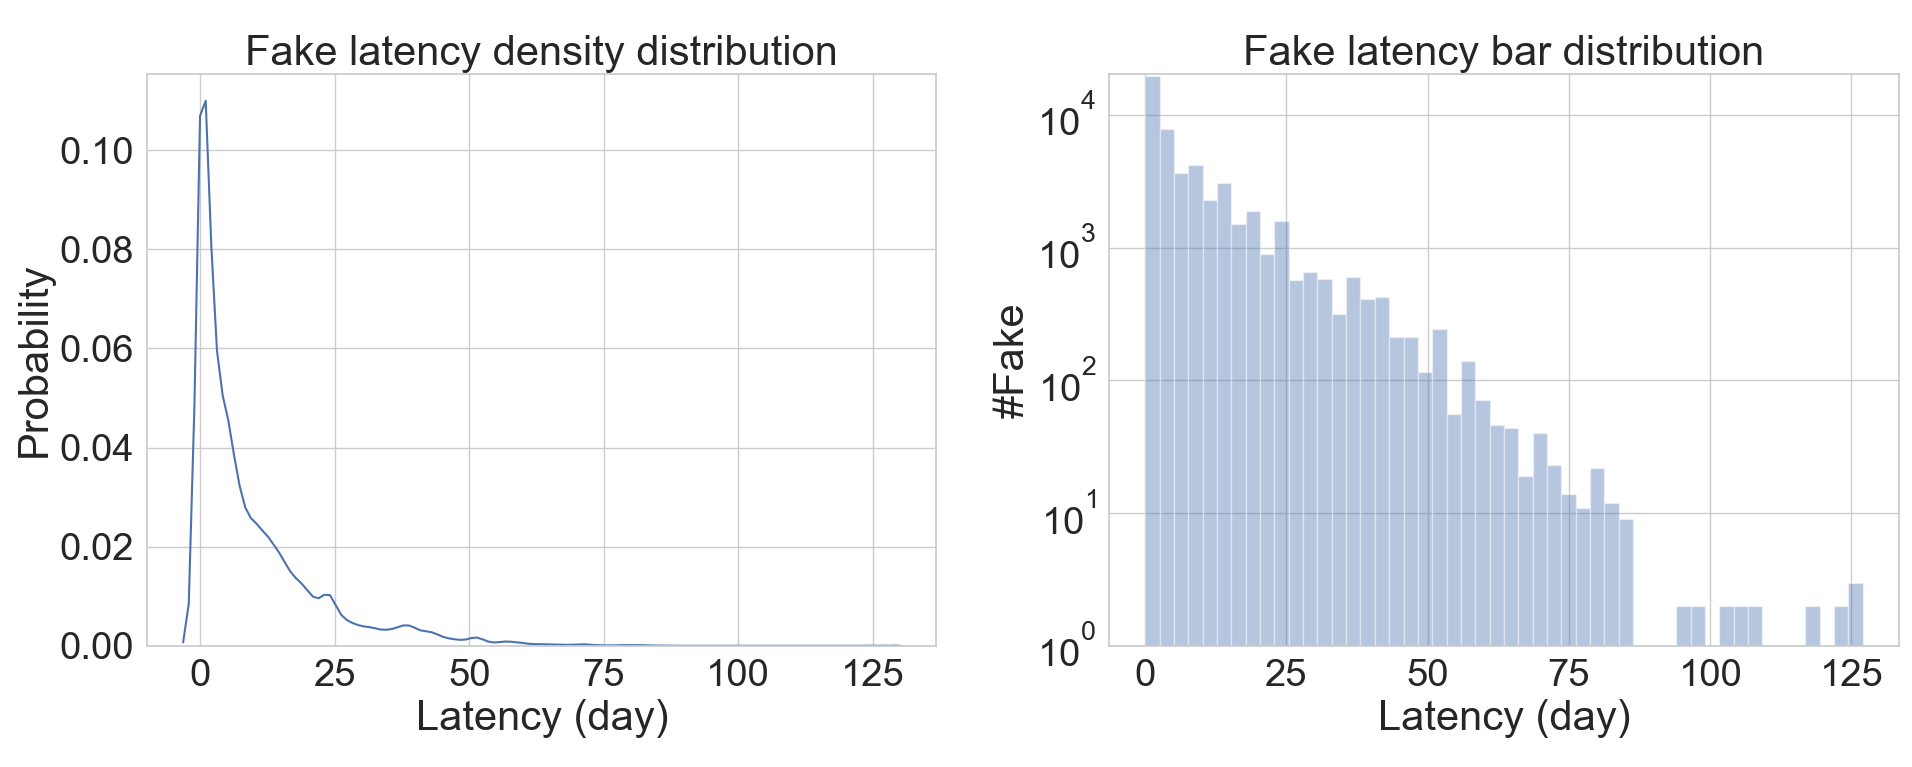
\includegraphics[width=\textwidth]{./Figures/edwin-Fake_latency_overall_distribution2.png}
%     \caption{仿冒延迟总体分布}
%     \label{fig:Fake_latency_overall_distribution}
% \end{figure}


% % Fig.~\autoref{fig:Fake_latency_overall_distribution} shows that most fake samples are published with the latency shorter than 20 days.
% 按照\autoref{fig:Fake_latency_overall_distribution}的结果,绝大多数仿冒样本在官方应用推出后的20天内就被发布了。
% % According to our statistics, 60\% of fake samples show up in 6 days after a new version of the official app is published.
% 根据本文的统计,有60\%仿冒应用在正版App被推出的6天内就被发布出来了。
% % This reveals a truth that fake developers are swift in action.
% 这表明仿冒开发者的行动十分迅速。

% 随着时间推移,仿冒应用这个灰色产业是否有过变迁?
% 本节对此提出了研究问题:

% % \noindent{\bf RQ 3.3} Is there a changing pattern of fake samples over time?
% {\bf RQ 3.3}:仿冒应用是否存在一个随着时间变化的模式?

% 本研究统计了不同时间段所搜集到的样本数量,得出了结果如下:

% % \noindent{\bf Answer to RQ 3.3.} Fig.~\autoref{fig:Number_per_quarter} shows the number of fake samples collected per quarter since the fourth quarter of 2015.
% {\bf RQ 3.3. 结果}\autoref{fig:Number_per_quarter}呈现了Janus自2015年第四季度起在每个季度爬取到的仿冒样本的总量。
% % Although a large number of new fake samples get released in every quarter, the figure shows a tendency that the total number of fake apps on markets is gradually decreasing by years.
% 尽管Janus每个季度都能爬取到新上架的大量仿冒样本,图表信息表明,市场上仿冒应用的总数正在呈现逐年减少的趋势。
% % Note that our statistics only focus on fake samples, consequently this phenomenon does not indicate the underground industry is turning down.
% 要注意的是,此处的统计仅仅针对仿冒应用。
% 因此这个现象并不表明移动黑灰产的发展具有萧条的趋势。
% % Instead, we suppose this is possibly caused by the reform of fake apps.
% 相反地,本文认为这个现象更有可能是由黑灰产内部改革而导致的。

% % On one hand, as stricter review schemes and stronger protection systems are applied on app stores, it's inevitable that fake apps in this study, become harder and harder to get on the shelf.
% 从一方面看,随着信息技术发展,应用市场逐渐配备上了更智能、严格而又强大的监管机制和安全系统,本研究中的仿冒应用开发者无疑更难以将仿冒的应用投放到市场上了。
% % On the other hand, the new generation of malicious software, such as ransomware~\cite{ransomware} is impacting the underground industry.
% 从另一方面看,新一代的恶意软件,比如WannaCry等勒索软件~\cite{ransomware}也正在影响着整个移动黑灰产工业。
% % Compare to fake apps, the new malicious apps are not only hard to defend (due to the innovative or even state-of-the-art techniques they utilize) but also extremely profitable.
% 与仿冒应用相比,这些新一代的恶意软件不仅更难以防范(传统的反病毒软件思路是提取已有恶意代码的特征,从而识别恶意行为,但这无法遏制新型的恶意行为),而且也似乎更容易能获取暴利。
% % Wannacry, a ransomware which was first spotted in the 2nd quarter of 2017, conquered tens of thousands of devices in a couple of weeks, which directly pulled up Bitcoin's price like a rocket~\cite{wannacry_bitcoin_news}.
% Wannacry作为一种新型恶意软件,自2017年第二季度被首次发现开始,就能在数周内攻克数以千万计的设备,并让比特币的价格像搭火箭一样直线飙升~\cite{wannacry_bitcoin_news}。
% % Afterward, in the first quarter of 2018, a burst of cryptomining malware on phones emerged~\cite{comodo_report}.
% 之后不久,在2018年的第一季度,移动设备上也爆发了一系列的加密采矿恶意软件~\cite{comodo_report}。
% % This may be the reason why the number of fake samples suffers two suddenly drops in the second quarter of 2017 and the first quarter of 2018, respectively.
% 所以,本研究有理由猜测2017年第二季度和2018年第一季度的仿冒应用上架数量下跌是受到了新形态黑灰产的冲击。
% 当然,证实这个猜想还需要采集更多数据、进行更深入的研究。

% \subsection{研究结果有效性分析}
% \subsection{案例 1. 持有官方应用证书的可疑样本}

% 在人工浏览数据时,本研究发现了一个具有可疑应用名的样本---该样本声称自己是一个``破解版''的应用。
% % Furthermore, we checked (1) if strange word (e.g., ``cracked") appears in our official samples' names, (2) whether or not an official app is signed by an official certificate from another developer, and (3) if one official sample has a suspicious package name.
% 因此,本研究针对所有69,614个持有官方证书的样本进行了以下筛选:
% \begin{enumerate}
%     \item 使用``破解''、``免费''等关键字搜索所有带正版证书的样本,筛选出带有可疑应用名的样本;
%     \item 筛选所持应用证书与原开发者不一致的样本;
%     \item 筛选出包名和同款App的多数样本不一致的样本。
% \end{enumerate}

% % Eventually we acquired 17 suspicious official samples, listed in table~\ref{table:suspicious_samples} are samples in each of these three kinds.
% 最终,本文获得了17个由正版开发者应用证书签署的可疑样本,其中三个样本的信息如\autoref{table:suspicious_samples}中所示,分别代表上述三项筛选得到的结果。
% 第一个名为\texttt{爱奇艺}的样本虽然由一个官方应用证书签名,但该应用证书和其他爱奇艺样本的却不一致。
% 对比之后,本研究发现该证书来自360手机助手,但360和爱奇艺并没有合作关系,因此这是个可疑的样本;
% 而第二个样本(\texttt{360手机助手})的可疑之处在于样本包名。多数\texttt{360手机助手}的包名为\emph{com.qihoo.appstore},也有少部分官方包名为\emph{com.qihoo.secstore},前者为\texttt{360手机助手}在国内第三方应用市场发行的应用包名,后者为Google Play官方应用市场上上架的包名。然而,其中一个使用了其官方应用证书签署的样本的包名却是\emph{com.kuyou.sdbgj.baidu},十分奇怪;
% 第三个样本则是在应用名中包含了``破解''字样。然而,正常的正版应用根本不会有这样的命名方式,所以本研究也认为这是一个可疑样本。


% % \textsc{Virustotal} reports that only 2 of the 17 samples are benign, 2 are PUP and the other 13 samples are all malicious.
% \textsc{Virustotal} 的检查结果显示,17个可疑样本中,只有2个是良性应用,2个是PUP,余下13个样本都被判定具有恶意行为。
% 进行后续分析时,相关样本已被剔除出正版样本集合。

% \begin{table*}[htbp]
%     \renewcommand{\arraystretch}{1}
%     \small
%     \centering
%     % \setlength{\belowcaptionskip}{-10pt}
%     \caption{持有官方应用证书的可疑样本}
%     \begin{tabular}{l l c c c c c c}
%         \toprule
%         {\bf 样本应用名}               & {\bf 样本SHA1码}                         & {\bf 可疑之处} \\
%         \midrule
%         % 爱奇艺 & b86c55a509e8293b24138b166e9ff410f39e84b5 & 可疑证书(360手机助手) \\
%         爱奇艺                         & b86c55a509e8293b24138b166e9ff410f39e84b5 & 可疑证书       \\
%         % 360手机助手 & 2bb43c53b86d204d0040a8af6cb2a09cf9e93bb7 & 可疑包名(com.kuyou.sdbgj.baidu) \\
%         \rowcolor{gray!15} 360手机助手 & 2bb43c53b86d204d0040a8af6cb2a09cf9e93bb7 & 可疑包名       \\
%         % Youku XL 破解版 & b55b7ef189d649aeb03443c5d1ab57c9031d624e & 可疑应用名(``破解版") \\
%         Youku XL 破解版                & b55b7ef189d649aeb03443c5d1ab57c9031d624e & 可疑应用名     \\
%         \bottomrule
%     \end{tabular}
%     \label{table:suspicious_samples}
% \end{table*}

% % Despite the possibility that these certificates were somehow leaked to the underground industry, it is more likely that some attackers penetrated the protection scheme.
% 鉴于这17个样本都是持有官方应用证书签名的,有理由怀疑有应用厂家不慎泄露了自己的安全密钥库,从而导致了这些样本的出现。
% 然而,如果真的是因为厂家泄露密钥库,一来很有可能会导致恶意开发者使用官方应用证书大量生产恶意应用,二来对应厂家也会出于安全考虑马上更换新的包名和应用证书。
% 本研究的数据并不支持以上猜想带来的两点结果,所以本文不认为这是由于应用证书泄露导致了这些可疑样本的产生。

% 除去这个可能性,本文认为更有可能的原因是某些仿冒应用开发者掌握了穿透/绕过Android系统签名机制的技术,从而产生了这些样本。

% % As far back as December 2017, Google had confirmed and revealed a backdoor on V1 signature scheme (CVE-2017-13156)~\cite{android_security_bulletin}, by which hackers can inject any content into an apk at will without modifying its certificate information.
% 时间回溯到2017年12月,Google确认并公布了V1版本应用签名机制的一个后门(CVE-2017-13156)~\cite{android_security_bulletin}。
% 通过这个后门,黑客可以在不修改APK包应用证书信息的情况下,向APK包里注入任意内容。
% % An alternative solution, V2 signature scheme, has been launched at least one year before that.
% 而早在这个漏洞被公布的至少一年之前,Google就已经发布了作为V1版签名机制的替代解决方案,也就是V2版应用签名机制。
% % In order to confirm if these apps are using the risky V1 scheme, we used a tool, apksigner, provided by Google to verify which signature schemes these samples are using.
% 这看起来十分有可能是导致这些可以样本产生的原因,某些恶意开发者利用了V1版本签名机制的漏洞,修改了APK包的基本信息。
% 为了确认这些样本是否采用了具有风险的V1版应用签名机制,本文使用了apksigner来检测这些样本使用的签名机制版本。
% apksigner是Google官方提供的一个命令行工具,它被集成在Android SDK中,既是APK包编译打包过程中为APK包进行数字签名的工具,也可以用来验证APK包使用的签名机制版本,又或者是验证APK的签名是否有效。

% % It ends up that all 17 samples are using V1 signature scheme.
% apksigner的结果显示,所有17个样本都只使用了V1版本的应用签名机制。
% % With actually knowing that V1 is no longer safe, developers still refuse to embrace the safer scheme, which is really disappointing.
% 在了解到V1版本签名机制已经不再安全的情况下,仍有部分开发者由于各种原因没有接受更新也更安全的签名方案,这个结果令人失望。

% \section{相关工作}


% \section{本章小结与实用建议}
% 本章先分别从\emph{仿冒应用的基本特征}、\emph{影响仿冒应用数量的因素}和\emph{仿冒应用的发展轨迹}三个不同视角对采集到的数据进行了分析,并在每个视角后的本节小结中概括了每个视角的结论,解读仿冒应用的特征。
% 在每个视角的解读之后,本章还从数据集中选出了一些较有代表性又或者反直觉的数据样本,提供了3个不同的案例分析,在为本文的发现提供有力支持之外,也揭示了更多仿冒应用开发者的行为,深化了对仿冒应用生态的了解。

% 回看三个案例,不难发现,仿冒应用开发者的确会抓住一切可能的机会,利用包括签名机制漏洞、市场审查机制缺陷在内的各种办法制作出仿冒甚至是恶意应用。
% 同时,本章的三个案例也说明了无论是开发人员还是应用市场,都应该在保护Android的软件安全方面上投入更大精力,从而更好地防范来自移动黑灰产的各种攻击。

% 在对仿冒应用进行全方位特征解读后,本文进一步进行了面向仿冒应用的排名欺检测,以探究两者之间是否存在联系。
% 相关研究由下一章呈现。



% \vspace{5mm}
% \noindent\fbox{
%     \parbox{0.95\linewidth}{
%         % \textbf{Remark 3}: Fake apps can be produced in a relatively short time, and the dropping number of fake samples by years suggests that they are mired in recession.
%         \textbf{本节小结}:仿冒应用可以在极短时间内被研发并上架,而仿冒样本逐年下降的新增量,也许表明了仿冒应用产业正在陷入衰退期,但这需要更多证据和研究证实。
%         % Besides, only a few fake certificates survive for a long time, confirming that markets' protection schemes do work to some extent.
%         此外,只有很小一部分的仿冒应用应用证书可以活跃很长的一段时间,这表明应用市场的保护监管机制在一定程度上的确能发挥作用,但案例数据同时表明,现有检测方法仍有不足。
%         另外,案例提供的数据也表示了应用市场之间缺乏交流恶意开发者/可疑开发者信息的平台。
%     }
% }

% \vspace{5mm}
% \noindent\fbox{
%     \parbox{0.95\linewidth}{
%         % \textbf{Remark 1}: Most certificates link with only a number of fake apps, which is highly possible to be a fake developers' evasive strategy.
%         \textbf{本节小结}: 绝大部分应用证书只与少数仿冒样本有所关联。这很可能是仿冒开发者规避市场监管机制采用的策略。
%         % Moreover, we observe that fake apps do tend to use official app names or names alike.
%         同时,本文也观测到仿冒应用倾向于于官方App相同或者是十分相似的应用名。
%         % Nonetheless, fake apps and official apps are not resemble in terms of package names or apk sizes, disclosing that repackaged apps are not mainstream in fake apps.
%         但是,仿冒样本和官方App在包名和APK包大小方面都不相似,这表明重打包应用在仿冒应用中并不普遍存在。
%         最后,如果良性应用的开发者不遵从最新的安全标准发布应用,可能会导致十分严重的安全问题。
%     }
% }

% % To this end, we can draw the following conclusions:
% 在这里,可以得到以下两个结论:
% \begin{itemize}
%     % (1) Even the leading app markets (and the top developers) are unqualified in detecting malicious apps.
%     \item 就算是领先的应用市场(和顶尖的开发者)在检测恶意应用方面也不能做到尽善尽美,而现有的检测方法也有所不足,未能及时地找出可疑的开发者;
%           % (2) Existing app markets lack information exchange on defending attacks from underground industry.
%     \item 从这个证书在多个市场都存在的现象,本研究推导,现有的应用市场缺乏有效的信息交换机制。
%           如果各个应用市场能建立一个互通信息的平台,分享可疑开发者/恶意开发者信息,那么将可以杜绝一部分恶意开发者在各个应用市场上到处流窜的现象。
% \end{itemize}